\documentclass[10pt,twocolumn,letterpaper]{article}

\usepackage{cvpr}
\usepackage{times}
\usepackage{epsfig}
\usepackage{graphicx}
\usepackage{amsmath}
\usepackage{amssymb}

\usepackage[top=0in, bottom=0.7in, left=0.7in, right=0.7in]{geometry} % Adjust margins here


\usepackage[breaklinks=true,bookmarks=false]{hyperref}

\cvprfinalcopy

\def\httilde{\mbox{\tt\raisebox{-.5ex}{\symbol{126}}}}

\setcounter{page}{1}
\begin{document}

\title{\begin{center}
    DeepDetect : Detect Fake and AI-generated Images
\end{center}
Mid-Semester Project Report}

\author{Himang Chandra Garg \qquad Dasari Sai Harsh \qquad Nishil Agarwal \qquad Piyush Narula\\
Indraprastha Institute of Information Technology, Delhi\\
{\tt\small \{himang22214, dasari22144, nishil22334, piyush22354\}@iiitd.ac.in}
}

\maketitle

\pagestyle{empty}

%-------------------------------------------------------------------------

\section{Abstract}

Our project seeks to address the critical issue of detecting deepfake images and AI-generated content, which have become increasingly sophisticated and challenging to distinguish from real media. 
The goal is to enhance the ability to discern genuine content from fabricated images, thereby reducing the potential for misinformation.

\section{Introduction}

\subsection{Problem Statement}

The recent rise in AI content, particularly deepfake images and videos, has raised serious concerns about the integrity of information online. 
This synthetic media is often indistinguishable from real content, hence making it very difficult for an average person to tell the truth—an aspect with large implications in public trust, privacy, and security.

%------------------------------------------------------------------------
\section{Literature Survey}
Detecting fake images with machine learning is a difficult and growing research field because image editing tools are becoming more accessible and user-friendly. Recent studies have focused on creating automated systems utilizing machine-learning methods in order to identify counterfeit images. This review of literature outlines the latest research in this area and addresses the difficulties and future paths ahead using the following 2 papers.
\subsection{\href{https://ijrpr.com/uploads/V4ISSUE4/IJRPR11629.pdf}{Detecting Fake Images Using Machine Learning}}
The paper "Detecting Fake Images Using Machine Learning" by Mr. Akash K, Miss. Ahalya K, Mr. Dhinesh N, Miss. Diya Shereef delves into strategies for detecting manipulated images using both traditional image processing and machine learning approaches. The writers suggest a combination model that uses CNNs to extract features like color patterns, texture, and statistical characteristics from images. Next, these characteristics are inputted into a classifier that differentiates between authentic and altered images. The suggested model attains high accuracy and can be utilized in social media content moderation, news verification, and forensic investigations.

\subsection{\href{https://www.researchgate.net/publication/375952278_Deep_Learning_for_Image_Authentication_A_Comparative_Study_on_Real_and_AI-Generated_Image_Classification}{Deep Learning for Image Authentication: A Comparative Study on Real and AI-Generated Image Classification}}
The effectiveness of deep learning models in differentiating real images from AI-generated ones is investigated in the paper "Deep Learning for Image Authentication: A Comparative Study on Real and AI-Generated Image Classification" by Gaye Ediboglu Bartos and Serel Akyol. The research is centered around two models: Residual Networks (ResNet) and Variational Autoencoders (VAEs). ResNet, renowned for its strong feature extraction abilities, reached an impressive 94\% accuracy in distinguishing between real and synthetic images in the CIFAKE dataset, comprising 60,000 real and 60,000 AI-generated images. On the other hand, VAEs, taking an anomaly detection stance, had a lower accuracy of 71\% because of their generative nature and less discriminative architecture. The paper highlights how crucial it is to tune hyperparameters, such as batch sizes and epochs, in order to improve model performance. The findings show that ResNet is better for image authentication tasks than VAEs, which had difficulty with the CIFAKE dataset's complexity. In summary, the study emphasizes the importance of choosing the right model and optimizing it for specific tasks to improve the detection of AI-generated images. It indicates that ResNet's discriminative capabilities make it the best option for these tasks.

\section{Dataset}
\section{Methodology}
\begin{figure}[h]
    \centering
    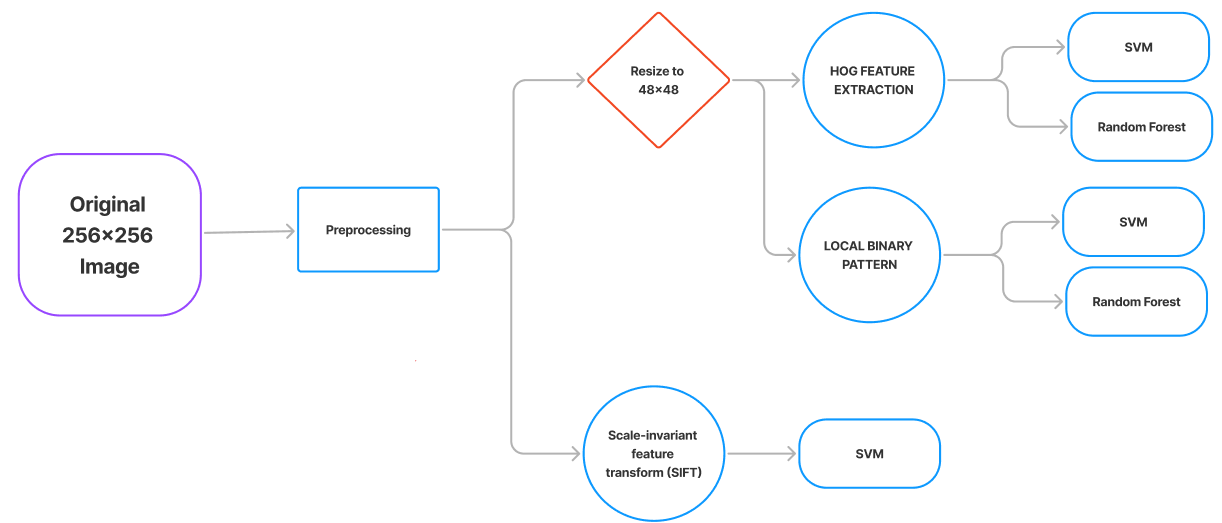
\includegraphics[width=\linewidth]{1.png}
    \caption{Workflow Flowchart}
\end{figure}
\subsection{Why Resize}
We resized the images to enhance computational efficiency and model performance. High-resolution images contain millio of pixels, leading to significant computational demands during training and inference. By reducing the image size, we lower the number of features, resulting in faster processing times and reduced memory usage. Additionally, traditional machine learning techniques, like SVMs and Random Forests, struggle with high-dimensional data due to the "curse of dimensionality," making it difficult to detect meaningful patterns.
\subsection{Pre-processing and Augmentation}

\subsection{Feature Extraction}
\textbf{Histogram of Oriented Gradients (HOG)} is a feature descriptor used in image processing and computer vision. It captures the distribution of gradients and edge directions within an image, effectively representing the shape and structure of objects. HOG is especially useful for object detection due to its invariance to changes in illumination and its ability to handle variations in object scale. 
A csv file containing the resized images is read and the HOG feature extraction is applied to each image and the resulting embedding is saved in a separate csv.

\textbf{Local Binary Patterns (LBP)} is also used as a feature extraction technique due to its effectiveness in capturing texture information. LBP encodes local spatial patterns and contrasts in images, making it suitable for differentiating between real and synthetic content. The code reads a CSV file containing flattened representations of 48x48 pixel images and their labels ("Real" or "Fake"). It applies LBP feature extraction to each image, generating a normalized histogram that represents the distribution of texture patterns. These extracted features are stored in a new DataFrame with the mapped labels and saved to a CSV file .

\textbf{Scale-Invariant Feature Transform (SIFT)} is a feature extraction method that identifies and describes local features in images. It detects keypoints across different scales and orientations, ensuring robustness to variations in image scale, rotation, and illumination. SIFT generates descriptors for these keypoints, which can be used for tasks such as image matching, object recognition, and classification.

In our project on detecting AI-generated images, SIFT is employed to extract distinctive features from the images. Its ability to capture detailed local information makes it effective for distinguishing between real and synthetic content.
\subsection{Model Training}
In our project, both Support Vector Machines (SVM) and Random Forests are employed for classification tasks using the features extracted from Histogram of Oriented Gradients (HOG) and Local Binary Patterns (LBP). For Random Forests, we follow the common practice of training with a subset of features, specifically using the square root of the total number of features \( \sqrt{m} \), which helps enhance model performance and reduces overfitting. Meanwhile, SVM is utilized for training on the features extracted from the Scale-Invariant Feature Transform (SIFT), leveraging its effectiveness in high-dimensional spaces to improve accuracy.

\section{Results and Analysis}
\subsection{HOG with SVM}

The classification model employing Histogram of Oriented Gradients (HOG) features with Support Vector Machines (SVM) achieved the following performance metrics:

\begin{itemize}
    \item \textbf{Accuracy:} 0.66, \textbf{Precision:} 0.68, \textbf{F1 Score:} 0.65, \textbf{ROC-AUC Score:} 0.73
\end{itemize}


The confusion matrix is as follows:

\[
\begin{array}{|c|c|c|}
\hline
& \text{Predicted Real} & \text{Predicted Fake} \\
\hline
\text{Actual Real} & 377 & 164 \\
\hline
\text{Actual Fake} & 206 & 343 \\
\hline
\end{array}
\]

The results indicate that the model has a balanced performance, with a slight edge in precision for the "Fake" class. The accuracy of 66\% suggests that the model is reasonably effective in distinguishing between real and fake images; however, there is room for improvement, particularly in recall for the "Fake" class, which could lead to missing genuine instances of AI-generated images.
The ROC-AUC score of 0.73 indicates a good capability in distinguishing between the two classes, reinforcing the model's utility for this task.


\subsection{Random Forest(with m=4) with LBP}

The classification model achieved an accuracy of 0.54, precision of 0.57, recall of 0.38, F1 score of 0.46, and ROC-AUC score of 0.73.

\begin{table}[h]
    \centering
    \begin{tabular}{|c|c|c|}
        \hline
        & \textbf{Predicted Real} & \textbf{Predicted Fake} \\ \hline
        \textbf{Actual Real} & 384 & 157 \\ \hline
        \textbf{Actual Fake} & 341 & 208 \\ \hline
    \end{tabular}
\end{table}

The Random Forest model using Local Binary Patterns (LBP) performed poorly, achieving an accuracy of only 0.54. With a precision of 0.57 for fake images and a recall of 0.38, the model struggles to effectively differentiate between real and fake images, resulting in high false positive and negative rates. The confusion matrix  highlights serious misclassification issues.

LBP may be limited by the small image size of 48x48 pixels, which restricts its ability to capture detailed texture information. Thus, the model's current configuration is inadequate for the task. 
\subsection{SVM with LBP}

Accuracy: 0.57, Precision: 0.62, Recall: 0.37, F1 Score: 0.46, ROC-AUC Score: 0.73

The SVM model utilizing Local Binary Patterns (LBP) performed poorly, achieving an accuracy of only 0.57. This reflects significant challenges in differentiating between real and fake images, as indicated by the low recall of 0.37, resulting in many missed detections of fake images. The confusion matrix shows that out of 549 fake images, only 201 were correctly classified. 

Since the Random Forests model exhibited suboptimal performance with Local Binary Patterns (LBP), following the same trend observed in the SVM results,t his suggests that LBP may not be well-suited for smaller images (48x48 pixels) and could benefit from larger image sizes to enhance feature extraction and overall classification accuracy.

\begin{table}[h]
    \centering
    \begin{tabular}{|c|c|c|}
        \hline
        & \textbf{Predicted Real} & \textbf{Predicted Fake} \\ \hline
        \textbf{Actual Real} & 420 & 121 \\ \hline
        \textbf{Actual Fake} & 348 & 201 \\ \hline
    \end{tabular}
\end{table}


\subsection{ SVM with SIFT}

The SVM model utilizing Scale-Invariant Feature Transform (SIFT) performed better than previous models, achieving an accuracy of 0.68. The precision for fake images was 0.61, indicating a reasonable level of correctness among the identified fake instances, while the recall score of 0.64 suggests that the model effectively captured a substantial number of fake images. Overall, the F1 score of 0.62 reflects a balanced performance between precision and recall.

\begin{table}[h]
    \centering
    \begin{tabular}{|c|c|c|}
        \hline
        & \textbf{Predicted Real} & \textbf{Predicted Fake} \\ \hline
        \textbf{Actual Real} & 392 & 233 \\ \hline
        \textbf{Actual Fake} & 208 & 366 \\ \hline
    \end{tabular}
\end{table}


\section{Conclusion}
\section{References}
\end{document}
